\documentclass[12pt]{article}
\usepackage[portuguese]{babel}
\usepackage{natbib}
\usepackage[export]{adjustbox}
\usepackage{float}
\usepackage{url}
\usepackage[utf8x]{inputenc}
\usepackage{mathtools}  
\usepackage{graphicx}
\graphicspath{images}
\usepackage{listings}
\usepackage[margin=2cm]{geometry}
\usepackage{wrapfig}
\renewcommand*{\thesubsubsection}{\alph{subsubsection}.}
\usepackage{multicol}
\usepackage{caption}

\begin{document}

\begin{titlepage}

\center % Center everything on the page

\newcommand{\HRule}{\rule{\linewidth}{0.4mm}} % Barra horizontal

\textsc{\LARGE Universidade do Minho}\\[0.5cm]  % Name of your university/college

\vspace{1cm}
\textsc{\large Licenciatura em Engenharia Informática}\\[1.5cm] % Nome do curso
\vspace{0.5cm}

\HRule \\[0.5cm]
{ \LARGE \bfseries } Redes de Computadores \\[0.5cm] % Título
{ \LARGE \bfseries } \textbf{Grupo 135} \\[0.5cm] % Grupo
\HRule \\[1cm]
\vspace{0.1cm}
 
\paragraph{}
\paragraph{}
\textsc{\Large \textbf{TP3: \textit{Link Layer}: Redes \textit{Ethernet} e Protocolo ARP}}\\[0.75cm] % Nome da UC
\vspace{2.5cm} % Autores
Joana Alves (A93290) \\ \vspace{3mm}
João Machado (A89510) \\ \vspace{3mm} 
Rui Armada (A90468) \\ \vspace{3mm}

\vspace{3cm}


\vspace*{\fill}

{\large Abril 2022}\\[2cm] % Data

\vfill % Fill the rest of the page with whitespace
\end{titlepage}








% ---------- QUESTÕES ---------



\section*{\hfil Questões e Respostas\hfil}



\section{Questão 3}
% Responda às perguntas seguintes com base no conteúdo da trama Ethernet que contém a mensagem de acesso ao servidor (HTTP GET encriptada).

\begin{figure}[H]
\centering
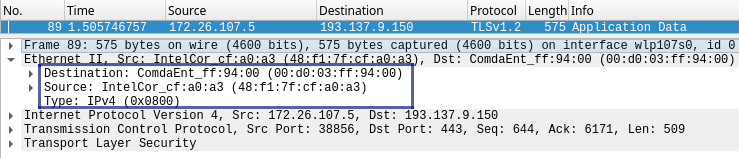
\includegraphics[width=500pt]{prints/Questao3/questao3.tramaClient.png}
\caption{Captura da Trama \textit{Ethernet} que contém mensagem de acesso.} \label{questao3-1}
\end{figure}


\subsubsection{Anote os endereços MAC de origem e de destino da trama capturada.}

    \par Estes endereços podem ser consultados no campo \textit{Source} e \textit{Destination}, respetivamente, no cabeçalho da trama \textit{Ethernet}, tal como se demonstra com a Figura \ref{questao3-1}:

    \begin{multicols}{2}
    \begin{itemize}
        \item MAC Origem: \textbf{48:f1:7f:cf:a0:a3}  
        \item MAC Destino: \textbf{00:d0:03:ff:94:00}
    \end{itemize}
    \end{multicols}
    




\paragraph{}
\subsubsection{Identifique a que sistemas se referem. Justifique.}

    \par O endereço MAC de origem refere-se à máquina nativa utilizada nesta questão, tendo esta o endereço IP 172.26.107.5. No caso do endereço MAC destino, este refere-se ao sistema destino do próximo salto na rede, isto é, ao \textit{router} de acesso ou \textit{default gateway}, uma vez que, contrariamente ao nível de rede (protocolo IP), o nível de ligação lógica vai recalculando \textbf{salto-a-salto} o endereço MAC destino contido na trama até chegar ao endereço coincidente com o endereço IP destino, neste caso, 193.137.9.150.




\paragraph{}
\subsubsection{Qual o valor hexadecimal do campo \textit{Type} da trama \textit{Ethernet}? O que significa?}

    \par O campo \textit{Type} tem como valor \textbf{0x0800}, que representa o protocolo \textit{IPv4}, ou seja, este campo indica qual o protocolo que está a ser encapsulado pela trama.




\subsubsection{Quantos \textit{bytes} são usados no encapsulamento protocolar, i.e. desde o início da trama até ao início dos dados do nível aplicacional (Application Data Protocol: http-over-tls)? Calcule e indique, em percentagem, a sobrecarga (\textit{overhead})
introduzida pela pilha protocolar}

    \begin{figure}[H]
    \centering
    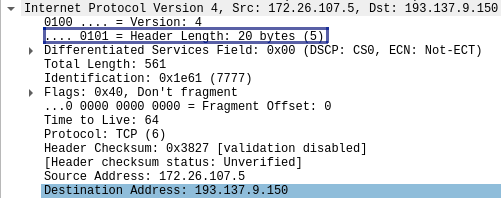
\includegraphics[width=280pt]{prints/Questao3/questao3-IP.png}
    \caption{Protocolo IP encapsulado.} \label{questao3-d-IP}
    \end{figure}
    
    \begin{figure}[H]
    \centering
    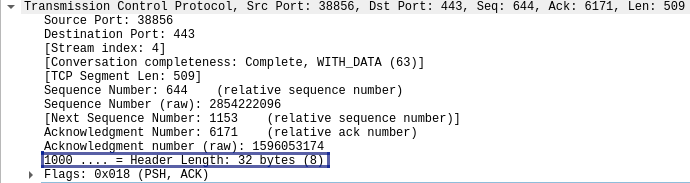
\includegraphics[width=380pt]{prints/Questao3/questao3-TCP.png}
    \caption{Protocolo TCP encapsulado.} \label{questao3-d-TCP}
    \end{figure}
    
    \paragraph{}
    \par Neste caso são vários os protocolos encapsulados pela trama \textit{Ethernet}, como, por exemplo, o protocolo IP (nível de rede) e TCP (nível de transporte). Assim, conseguimos somar o tamanho de todos os cabeçalhos (\textit{Ethernet}, IP, TCP) utilizados para encapsular os dados do nível aplicacional (\textit{Application Data Protocol}), obtendo o seguinte resultado: 
    
    \begin{align*}
        {14 \:(\textit{Ethernet}) + 20 \:(IP) + 32 \:(TCP) = \textbf{66}\:\textit{bytes}}
    \end{align*} 

    
    
    \par Pelos cálculos, obtivemos um total de 66 \textit{bytes} de encapsulamento protocolar. Relativamente à \textbf{sobrecarga} (\textit{overhead}), esta terá o valor de: 
    
    \begin{align*}  
        \frac{66\:(\textit{headers})}{575\:(tamanho\:total)*} = \textbf{11,5}\:\%  
    \end{align*}  
    
    
    \par \textbf{* NOTA:} O tamanho total da trama com a inclusão dos cabeçalhos foi verificada na Figura \ref{questao3-1} na primeira linha referente à informação do \textit{Frame}.  






% A seguir responda às seguintes perguntas, baseado no conteúdo da trama Ethernet que contém o primeiro byte da resposta HTTP proveniente do servidor
\subsubsection{Qual é o endereço \textit{Ethernet} da fonte? A que sistema de rede corresponde? Justifique.}

    \begin{figure}[H]
    \centering
    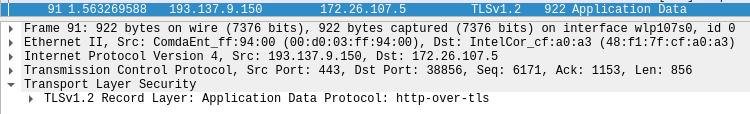
\includegraphics[width=500pt]{prints/Questao3/questao3-respostaServer.png}
    \caption{Captura da Trama \textit{Ethernet} de resposta.} \label{questao3-resposta1}
    \end{figure}


    \par O endereço \textit{Ethernet} da fonte é \textbf{00:d0:03:94:00} que corresponde ao sistema que na trama capturada nas alíneas anteriores estava no endereço MAC destino, ou seja, o \textit{router} de acesso ou \textit{default gateway} (último salto na rede até à máquina nativa).





\subsubsection{Qual é o endereço MAC do destino? A que sistema corresponde?}

    \par O endereço MAC destino é \textbf{48:f1:7f:cf:a0:a3} e corresponde à máquina nativa utilizada para responder a esta questão. Podemos confirmar pela análise à trama utilizada nas alíneas anteriores, pois este endereço corresponde ao endereço MAC origem da mesma.




\subsubsection{Atendendo ao conceito de desencapsulamento protocolar, identifique os vários protocolos contidos na trama recebida.}

    \paragraph{}
    \par Segundo o modelo OSI, existem sete camadas protocolares, onde podemos denotar a independência e modularidade entre as mesmas. Isto é, cada camada é desenvolvida de forma independente das outras, tendo responsabilidades e funcionalidades distintas, fornecendo serviços à camada diretamente acima e utilizando serviços da camada diretamente abaixo.
    
    \par Assim, cada nível protocolar utiliza uma PDU (\textit{Protocol Data Unit}) única com informações pertinentes que apenas consegue ser interpretada e manipulada pelas camadas homólogas. Desta forma, quando uma camada utiliza os serviços da camada de baixo, a informação que é transportada para o nível inferior vai ser encapsulada pelo mesmo, ou seja, por exemplo, a camada A envia os seus dados para a camada B (nível inferior) em formato \textit{PDU-A}, que, por sua vez, são encapsulados pela camanda B para \textit{PDU-B}.
    
    \par Em consequência, conforme os dados vão sendo enviados para as camadas inferiores, existe um encapsulamento protocolar sucessivo até ser atingido o nível mais baixo. Como tal, no caso em estudo, podemos denotar os vários protocolos encapsulados:

    
    \begin{figure}[H]
    \centering
    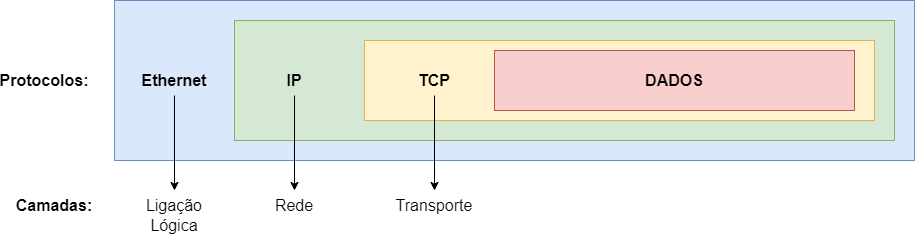
\includegraphics[width=450pt]{prints/Questao3/encapsulamento.png}
    \label{questao3-resposta2}
    \end{figure}




\section{Questão 4}

\subsubsection{Observe o conteúdo da tabela ARP. Diga o que significa cada uma das colunas.}

    \begin{figure}[H]
    \centering
    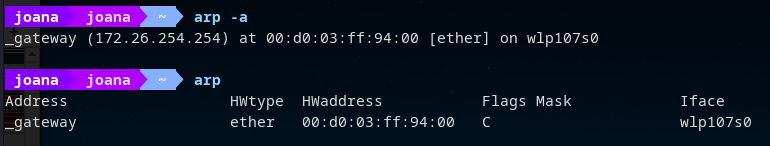
\includegraphics[width=350pt]{prints/Questao4/questao4-ArpTABLE.png}
    \caption{Tabela ARP.} \label{questao4-ARPRequest1}
    \end{figure}
    
    \par Uma tabela ARP é um método de armazenamento de informações descobertas através do protocolo ARP. É usada para registar os pares correspondentes de endereços MAC e endereços IP de dispositivos conectados a uma rede. Cada dispositivo conectado possui a sua própria tabela ARP, que, tal como referido acima, é responsável por armazenar os pares de endereços com os quais um determinado dispositivo já comunicou. Assim, apresentamos uma descrição das várias colunas presentes na tabela ARP.
    
    \begin{center}
        \begin{tabular}{|c|c|}
        \hline
            \cline{1-2}
            Coluna & Descrição  \\
            \hline \hline
            Address & endereço IP destino na rede\\
            HWtype & tipo de \textit{hardware} \\
            HWaddress & endereço MAC do \textit{hardware}\\
            Flags* & informação sobre a entrada \\
            Mask & máscara a aplicar ao endereço IP \\
            Iface & interface de saída \\
            \cline{1-2}
        \end{tabular}
    \end{center}
    
    \par \textbf{*} Neste caso, o valor da coluna é 'C'. Este tipo de entrada é visto quando as entradas são dinamicamente aprendidas pelo protocolo ARP.


    
    





\subsubsection{Qual é o valor hexadecimal dos endereços origem e destino na trama Ethernet que contém a mensagem com o pedido ARP (ARP Request)? Como interpreta e justifica o endereço destino usado?}

    \begin{figure}[H]
    \centering
    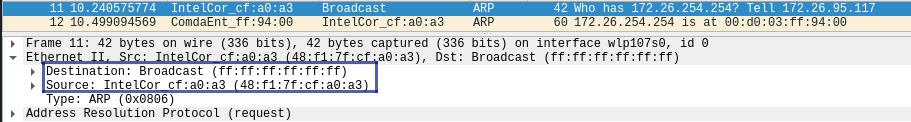
\includegraphics[width=500pt]{prints/Questao4/questao4-firstARP.png}
    \caption{Captura da Trama \textit{Ethernet} com pedido ARP.} \label{questao4-ARPRequest2}
    \end{figure}
    
    \begin{multicols}{2}
    \begin{itemize}
        \item MAC Origem: \textbf{48:f1:7f:cf:a0:a3}  
        \item MAC Destino: \textbf{ff:ff:ff:ff:ff:ff}
    \end{itemize}
    \end{multicols}


    \par A utilização do endereço MAC destino com o valor dos \textit{bits} todos a 1, é uma particularidade do protocolo ARP, isto é, como apagamos a \textit{cache} da tabela ARP, esta não tem qualquer informação de tradução e correspondência entre endereços IP e endereços MAC. Assim, quando, como neste caso, queremos enviar algum pacote para outro dispositivo, temos de primeiro descobrir o seu endereço MAC. Este problema é solucionado colocando o endereço MAC destino com todos os \textit{bits} a 1, representando uma mensagem em \textbf{\textit{broadcast}} (contendo o endereço IP do dispositivo alvo). 
    \par O modo de funcionamento pode ser caracterizado como uma difusão do pedido de \textit{broadcast} do nosso dispositivo por todos os nodos da mesma rede local até encontrar o aparelho que contém o mesmo endereço IP que o endereço IP destino do pedido. De seguida, o aparelho destino (alvo) envia uma resposta (ARP \textit{reply}) à nossa máquina contendo o seu endereço MAC.



\subsubsection{Qual o valor hexadecimal do campo tipo da trama Ethernet? O que indica?}

    \par O valor do campo \textit{type} do cabeçalho da trama \textit{Ethernet} é \textbf{0x0806} que indica que o protocolo encapsulado pela trama é o protocolo ARP.




\subsubsection{Como pode confirmar que se trata efetivamente de um pedido ARP? Identifique que tipo de endereços estão contidos na mensagem ARP? Que conclui?}

    \begin{figure}[H]
    \centering
    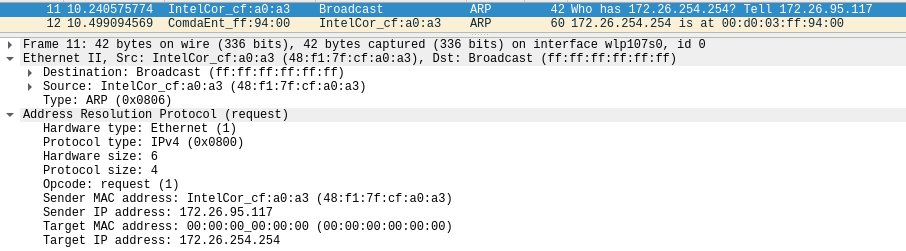
\includegraphics[width=500pt]{prints/Questao4/questao4-firstARP.png.png}
    \caption{Conteúdo ARP.} \label{questao4-ARPRequest-Extended}
    \end{figure}
    
    \paragraph{}
    \par Podemos confirmar que se trata de um pedido ARP pela análise do conteúdo da mensagem ARP, nomeadamente no valor do campo \textit{\textbf{Opcode}}. Este campo indica que tipo de mensagem ARP estamos a tratar, tendo, neste caso, o valor 1 que corresponde a um \textit{\textbf{request}}.
    
    \par Os endereços contidos na mensagem ARP são endereços MAC e IP dos sistemas de origem e destino, ou seja, para cada sistema está indicado o seu endereço IP e correspondente endereço MAC. No entanto, como podemos ver pela Figura \ref{questao4-ARPRequest-Extended}, esta possui o valor do endereço MAC destino (\textit{Target MAC Address}) a zeros. Isto acontece porque, como referido anteriormente, o endereço MAC destino é uma incógnita, sendo, exatamente, o que o protocolo  ARP está a tentar resolver.




\subsubsection{Explicite que tipo de pedido ou pergunta é feita pelo host de origem.}

    \par O \textit{host} de origem envia um pedido (ARP \textit{request}) a todos os nodos presentes na mesma LAN com o objetivo de obter uma resposta (ARP \textit{reply}) do sistema cujo endereço IP corresponde ao endereço IP destino presente na mensagem enviada, contendo esta, também, o endereço MAC do sistema alvo.


\subsubsection{Localize a mensagem ARP que é a resposta ao pedido ARP efetuado. (1) Qual o valor do campo ARP \textit{opcode}? O que especifica? (2) Em que campo da mensagem ARP está a resposta ao pedido ARP? }

    \begin{figure}[H]
    \centering
    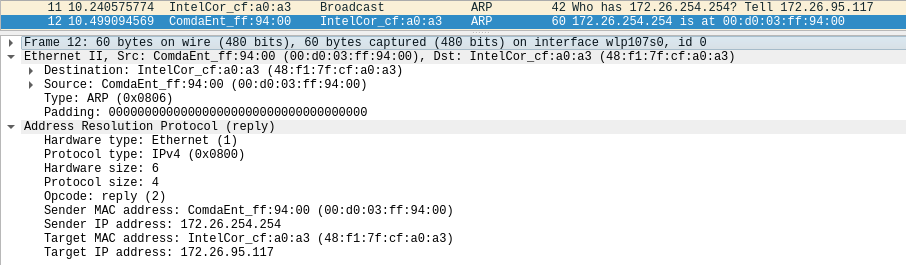
\includegraphics[width=500pt]{prints/Questao4/questao4-responseARP.png}
    \caption{Captura da Trama \textit{Ethernet} com resposta ARP.} \label{questao3-ARPResponse}
    \end{figure}
    
    \
    \par \textbf{(1)} O valor do campo \textit{Opcode} é 2 que corresponde a uma mensagem do tipo \textit{\textbf{ARP reply}}, ou seja, é uma mensagem de resposta a um pedido (\textit{request}) ARP.
    
    \par \textbf{(2)} O conteúdo da resposta ao pedido ARP está presente no campo \textbf{\textit{Sender MAC Address}}, onde podemos denotar a introdução de um endereço MAC válido, contrariamente ao presente no campo \textit{Target MAC Address} do ARP \textit{request} analisado anteriormente.




\newpage
\subsubsection{Na situação em que efetua um ping a outro host, assuma que este está diretamente ligado ao mesmo router, mas noutra subrede, e que todas as tabelas ARP se encontram inicialmente vazias. Esboce um diagrama em que indique claramente, e de forma cronológica, todas as mensagens ARP e ICMP trocadas, até à recepção da resposta ICMP do host destino.}


    \begin{figure}[H]
    \centering
    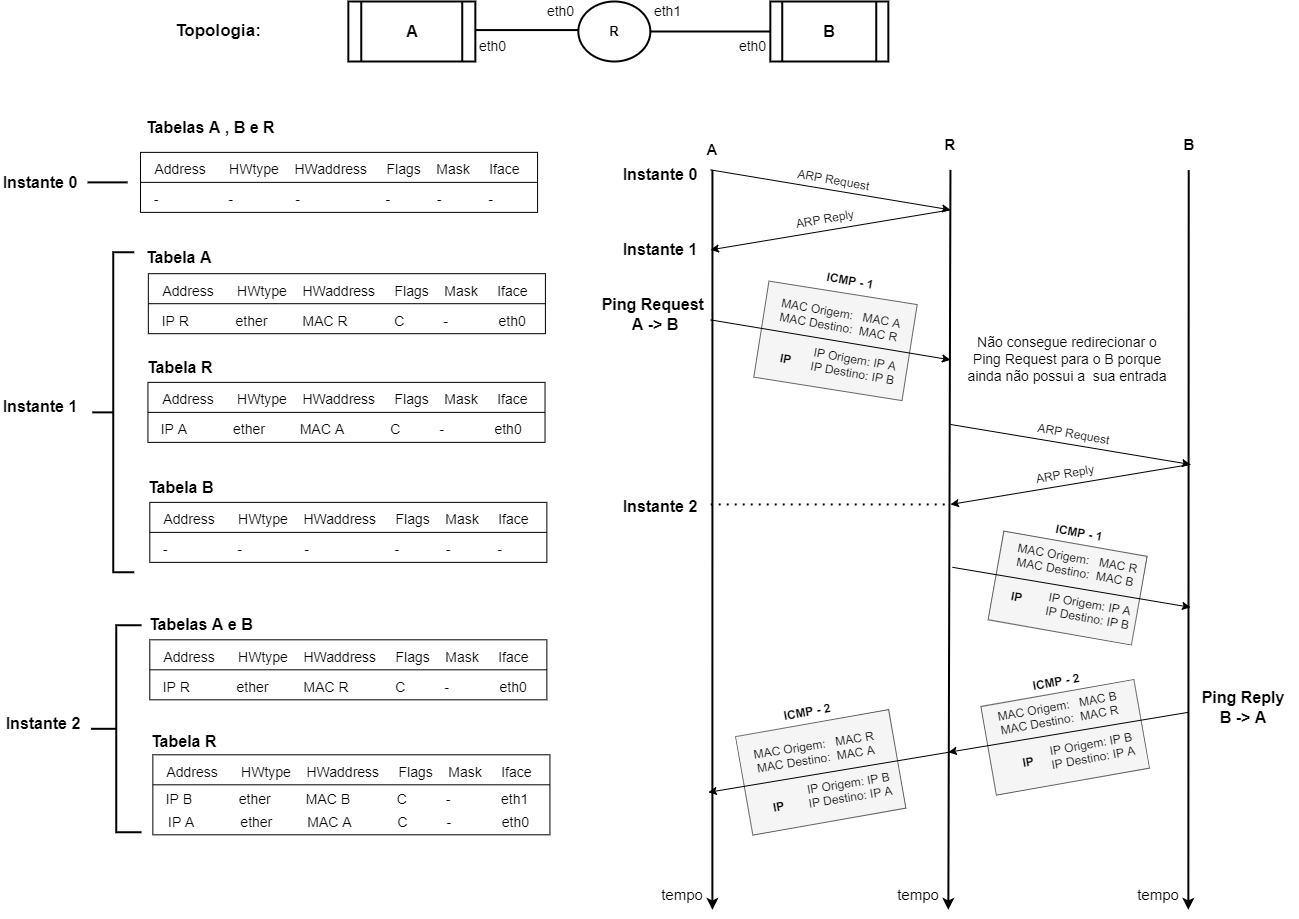
\includegraphics[width=\linewidth]{prints/Questao5/diagramaNOVO.png}
    \end{figure}


\section{Questão 5}

\subsubsection{Através da opção tcpdump verifique e compare como flui o tráfego nas diversas interfaces do dispositivo de interligação no departamento A (LAN partilhada) e no departamento B (LAN comutada) quando se gera tráfego intra-departamento (por exemplo, fazendo ping IPaddr da Bela para Monstro, da Jasmine para o Alladin, etc.) Que conclui?}

    \begin{figure}[H]
    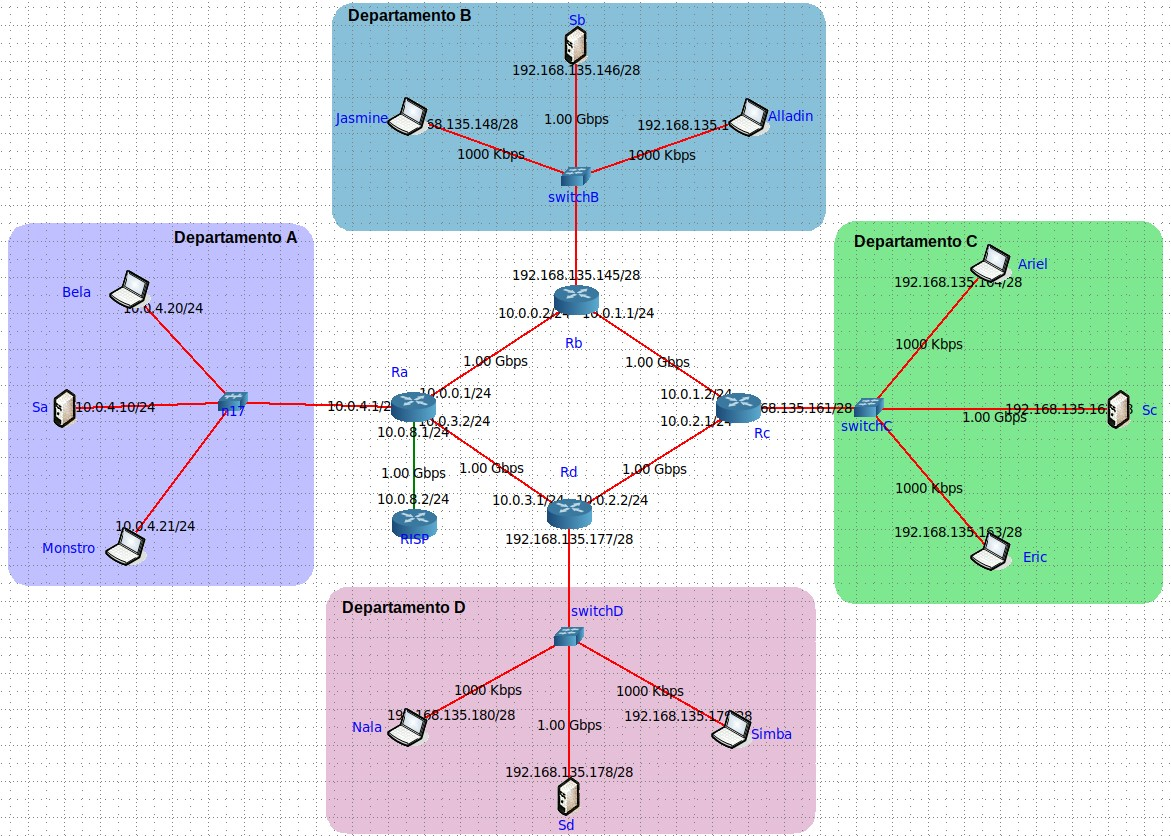
\includegraphics[width=\linewidth]{prints/Questao5/topologia.jpg}
    \caption{Topologia com o \textit{hub} adicionado.} 
    \label{questao5-topologia}
    \end{figure}
    

    \par Como podemos ver pela Figura \ref{questao5-topologia}, os endereços IP dos dispositivos Bela, Monstro e servidor Sa foram alterados em consequência da inserção do \textit{hub} e remoção do \textit{switch}. No entanto, o grupo optou por não voltar a alterar os endereços para os obtidos com o exercício de \textit{subnetting} do trabalho prático anterior, uma vez que não não iria alterar o comportamento esperado neste exercício em particular. Os testes foram realizados da seguinte forma: executou-se um \textit{ping} de um \textit{host} A para outro \textit{host} B e executou-se o comando \textit{tcpdump} num \textit{host} C não envolvido na comunicação do \textit{ping}. Assim, no \textbf{departamento A} executamos o comando \textit{ping} do \textit{host} Monstro para Bela e o comando \textit{tcpdump} no servidor Sa. No caso do \textbf{departamento B}, executamos o comando \textit{ping} do \textit{host} Alladin para Jasmine e o comando \textit{tcpdump} no servidor Sb. Por fim, obtivemos os seguintes resultados com os vários comandos:
            
            
    \begin{minipage}{0.5\linewidth}
        \centering
            \begin{figure}[H]
            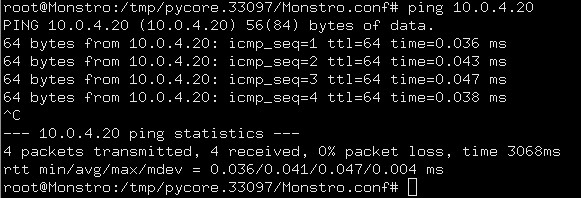
\includegraphics[width=\linewidth]{prints/Questao5/A-Monstro-Bela.jpg}
            \caption{Ping do \textit{host} Monstro para Bela.} \label{questao5-ping-A}
            \end{figure}
    \end{minipage}
    \begin{minipage}{0.5\linewidth}
        \centering
            \begin{figure}[H]
            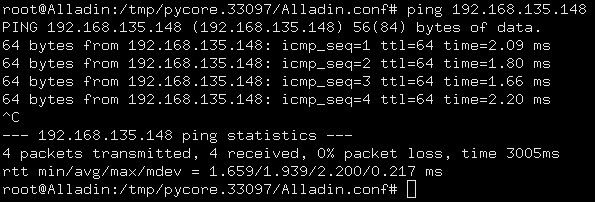
\includegraphics[width=\linewidth]{prints/Questao5/B-Alladin-Jasmine.jpg}
            \caption{Ping do \textit{host} Alladin para Jasmine.} \label{questao5-ping-B}
            \end{figure}
    \end{minipage}

    \paragraph{}
    \paragraph{}
    \begin{figure}[H]
    \centering
    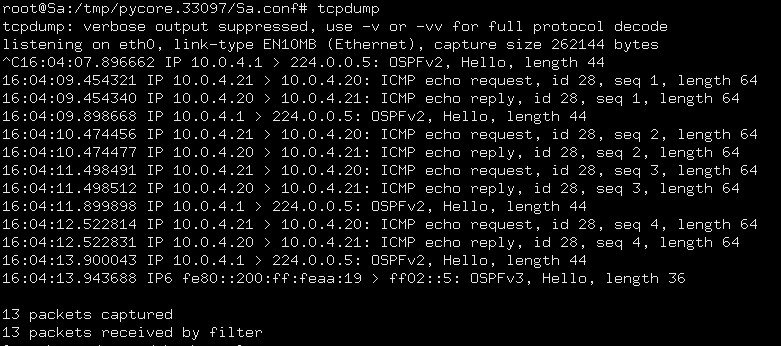
\includegraphics[width=400pt]{prints/Questao5/A-Sa.jpg}
    \caption{Comando \textit{tcpdump} no servidor Sa (LAN partilhada).} \label{questao5-tcpdump-A}
    \end{figure}
    
    \begin{figure}[H]
    \centering
    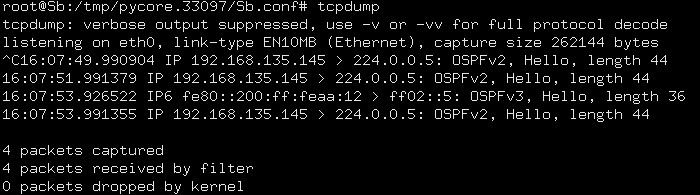
\includegraphics[width=400pt]{prints/Questao5/B-Sb.jpg}
    \caption{Comando \textit{tcpdump} no servidor Sb (LAN comutada).} \label{questao5-tcpdump-B}
    \end{figure}
    
    
    
    \par Existem várias diferenças entre \textit{hubs} e \textit{switches}, sendo a mais distinta a camada protocolar onde operam, isto é, o \textit{hub} opera ao nível físico enquanto que os \textit{switches} operam na camada de ligação lógica.
    Para além disto, os \textit{\textbf{hubs}} são dispositivos que repetem o sinal que chega através de uma porta de entrada para todas as outras portas, isto é, difundem o sinal por todas as interfaces que possuem.
    No que toca aos \textit{\textbf{switches}}, estes, com a ajuda de uma tabela de \textit{switching} (comutação), comutam as tramas para a interface de saída apropriada. No entanto, caso se depare com uma trama que não tem um endereço que conste na tabela, este difunde a trama por todas as suas interfaces, obtendo, neste caso em específico, um comportamento semelhante ao \textit{hub}.

    \par Assim, e tendo estas distinções em mente, conseguimos de imediato notar diferenças no resultado do comando \textit{tcpdump} nas duas situações. Na \textbf{LAN partilhada}, o terceiro \textit{host} não envolvido diretamente na comunicação também recebeu os pacotes, provando assim a particularidade dos \textit{hubs} no que toca à difusão das comunicações por todas as portas dos mesmos.
    No caso da \textbf{LAN comutada}, denotamos que o resultado da captura é vazio no que toca a pacotes relacionados com a comunicação derivada do comando \textit{ping}, provando assim a diferença de comportamento do \textit{switch} com o \textit{hub}, pois o tráfego é comutado para as interfaces devidas, não sendo difundido pela rede.




%\newpage
\subsubsection{Construa manualmente a tabela de comutação do switch do Departamento B, atribuindo números de porta à sua escolha.}

    \paragraph{}
    \par Para obtermos os endereços MAC dos vários sistemas diretamente ligados ao \textit{switch}, executamos o comando \textit{\textbf{ifconfig -a}}. Assim, obtivemos os seguintes endereços, notando que no \textit{router} o endereço da interface \textit{eth2} corresponde à interface de ligação ao \textit{switch}.

    \begin{minipage}{0.5\linewidth}
        \centering
            \begin{figure}[H]
            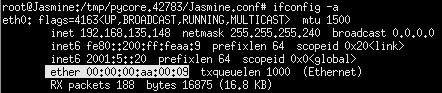
\includegraphics[width=\linewidth]{prints/Questao5/Jasmine.jpg}
            \caption{Endereço MAC Jasmine.} \label{questao5-MAC-Jasmine}
            \end{figure}
    \end{minipage}
    \begin{minipage}{0.5\linewidth}
        \centering
            \begin{figure}[H]
            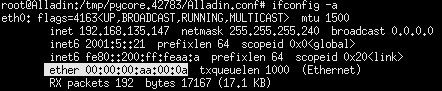
\includegraphics[width=\linewidth]{prints/Questao5/Alladin.jpg}
            \caption{Endereço MAC Alladin.} \label{questao5-MAC-Alladin}
            \end{figure}
    \end{minipage}
    
    \begin{minipage}{0.5\linewidth}
        \centering
            \begin{figure}[H]
            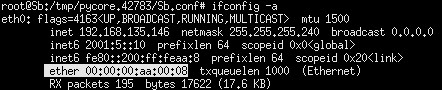
\includegraphics[width=\linewidth]{prints/Questao5/Servidor.jpg}
            \caption{Endereço MAC Servidor.} \label{questao5-MAC-Servidor}
            \end{figure}
    \end{minipage}
    \begin{minipage}{0.5\linewidth}
        \centering
            \begin{figure}[H]
            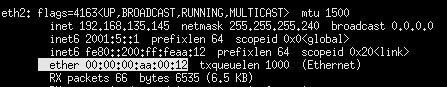
\includegraphics[width=\linewidth]{prints/Questao5/Router.jpg}
            \caption{Endereço MAC Alladin.} \label{questao5-MAC-Router}
            \end{figure}
    \end{minipage}
    
    \paragraph{}
    \par Após obtermos os endereços MAC, desenvolvemos um esboço da topologia da subrede do Departamento B (incluindo o \textit{router}) para assim termos uma visão simplificada dos sistemas integrantes. Como tal, obtivemos a seguinte tabela de comutação:
    
    \begin{figure}[H]
    \centering
    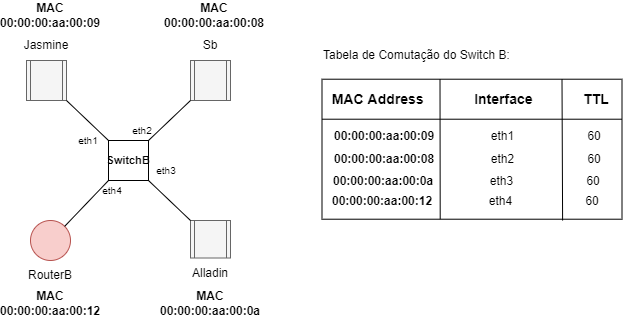
\includegraphics[width=450pt]{prints/Questao5/switch.png}
    \label{questao5-switchTable}
    \end{figure}






\section{Conclusão}
    
    \par Com a conclusão deste guião prático, encontramo-nos, em geral, satisfeitos com o trabalho desenvolvido, tendo alcançado todos os objetivos propostos pelos docentes no enunciado.
    
    \par Em particular, este trabalho prático incidiu sobre a resolução de vários exercícios e problemas da área de redes, nomeadamente a camada de ligação lógica. Assim, o grupo teve a oportunidade de aprofundar os seus conhecimentos em estudo de endereços MAC, funcionamento do protocolo \textit{Ethernet} e interpretação do protocolo ARP. Para além disso, mais uma vez, foi necessário o manuseamento da ferramenta \textit{wireshark}, provando, novamente, a sua utilidade prática no contexto de análise de tráfego. 

    \par Em suma, a construção e desenvolvimento deste trabalho prático permitiu a todo o grupo aprofundar os seus conhecimentos no que toca à camada de ligação lógica, atingindo uma ampla percepção de alguns assuntos englobados pela mesma.

\end{document}